\documentclass[10pt]{article}
\usepackage{fullpage,enumitem,amsmath,amssymb,graphicx,listings,tikz,bbm,xcolor}
\setlength{\parindent}{0pt}

\begin{document}

\begin{center}
{\Large \textbf{Homework 6: Scheduling}}

\begin{tabular}{rl}
\\
Course: & CS 221 Spring 2019 \\
Name: & Bryan Yaggi
\end{tabular}
\end{center}

What courses should you take in a given quarter? Answering this question requires balancing your interests, satisfying prerequisite chains, graduation requirements, availability of courses; this can be a complex tedious process. In this assignment, you will write a program that does automatic course scheduling for you based on your preferences and constraints. The program will cast the course scheduling problem (CSP) as a constraint satisfaction problem (CSP) and then use backtracking search to solve that CSP to give you your optimal course schedule.
\smallskip

You will first get yourself familiar with the basics of CSPs in Problem 0. In Problem 1, you will implement two of the three heuristics you learned from the lectures that will make CSP solving much faster. In Problem 2, you will add a helper function to reduce n-ary factors to unary and binary factors. Lastly, in Problem 3, you will create the course scheduling CSP and solve it using the code from previous parts. 

\section*{\normalsize Problem 0: CSP Basics}

\begin{enumerate}[label=(\alph*)]

  \item Let's create a CSP. Suppose you have $n$ light bulbs, where each light bulb $i = 1, \dots, n$ is initially off. You also have $m$ buttons which control the lights. For each button $j = 1, \dots, m$, we know the subset $T_j \subseteq \{1, \dots, n\}$ of light bulbs that it controls. When button $j$ is pressed, it toggles the state of each light bulb in $T_j$ (For example, if $3 \in T_j$ and light bulb 3 is off, then after the button is pressed, light bulb 3 will be on, and vice versa).
  
  Your goal is to turn on all the light bulbs by pressing a subset of the buttons. Construct a CSP to solve this problem. Your CSP should have $m$ variables and $n$ constraints. For this problem only, you can use n-ary constraints. Describe your CSP precisely and concisely. You need to specify the variables with their domain, and the constraints with their scope and expression. Make sure to include $T_j$ in your answer.
  
  There are $m$ variables, one for each button. The domain consists of 1 or 0, indicating whether the button is pressed or not.
  $$X = (X_1, \dots, X_m), where \ X_j \in \{0, 1\}$$
  
  There are $n$ factors, one for each light. The factor will be 1 if the number of pressed buttons controlling the light is odd.
  $$f_i = \mathbbm{1}\left[\left(\sum_{j : i \in T_j}^{m} X_j \right) \mod 2\right]$$
  
  \item Let's consider a simple CSP with 3 variables and 2 binary factors:
  
  \begin{center}
	  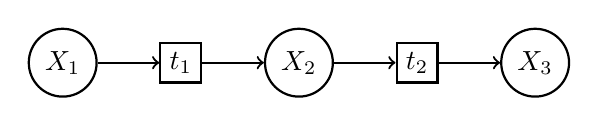
\begin{tikzpicture}
			\begin{scope}[every node/.style={circle,thick,draw}]
	    		\node (X1) at (3,0) {$X_1$};
	    		\node (X2) at (6,0) {$X_2$};
	    		\node (X3) at (9,0) {$X_3$};
			\end{scope}
			\begin{scope}[every node/.style={rectangle,thick,draw}]
	    		\node (t1) at (4.5,0) {$t_1$};
	    		\node (t2) at (7.5,0) {$t_2$};
			\end{scope}
	
			\begin{scope}[every edge/.style={draw=black,thick}]
				\path [->] (X1) edge node {} (t1);	    		
	    		\path [->] (t1) edge node {} (X2);
	    		\path [->] (X2) edge node {} (t2);
	    		\path [->] (t2) edge node {} (X3);
			\end{scope}
		\end{tikzpicture}
	\end{center}
	
	where $X_1, X_2, X_3 \in \{ 0, 1 \}$ and $t_1, t_2$ are XOR functions (that is $t_1(X) = X_1 \oplus X_2$ and $t_2(X) = X_2 \oplus X_3$).
	
	\begin{enumerate}[label=\roman*.]
		\item How many consistent assignments are there for this CSP?
		
		\begin{tabular}{c c c c c c}
		$X_1$ & $X_2$ & $X_3$ & $t_1$ & $t_2$ & $weight$\\
		\hline
  		$0$ & $0$ & $0$ & $0$ & $0$ & $0$\\
  		$1$ & $0$ & $0$ & $1$ & $0$ & $0$\\
  		$0$ & $1$ & $0$ & $1$ & $1$ & $1$\\
  		$1$ & $1$ & $0$ & $0$ & $1$ & $0$\\
  		$0$ & $0$ & $1$ & $0$ & $1$ & $0$\\
  		$1$ & $0$ & $1$ & $1$ & $1$ & $1$\\
  		$0$ & $1$ & $1$ & $1$ & $0$ & $0$\\
  		$1$ & $1$ & $1$ & $0$ & $0$ & $0$\\
  		\end{tabular}
  		
  		There are 2 consistent assignments: $x = \{ X_1 = 0, X_2 = 1, X_3 = 0 \}$ and $x = \{ X_1 = 1, X_2 = 0, X_3 = 1 \}$.
		
		\item To see why variable ordering is important, let's use backtracking search to solve the CSP without using any heuristics (MCV, LCV, AC-3) or lookahead. How many times will \texttt{backtrack()} be called to get all consistent assignments if we use the fixed ordering $X_1, X_3, X_2$? Draw the call stack for \texttt{backtrack()}. (You should use the Backtrack algorithm from the slides. The initial arguments are $x = \emptyset, w = 1$, and the original Domain.)
		
		In the code, this number will be stored in \texttt{BacktrackingSearch.numOperations}.
		
		Use domain ordering $Domain = \{ 0, 1 \}$. The top of the stack is on the bottom.
		
		\begin{tabular}{l}
		\textcolor{black}{\texttt{backtrack($x = \emptyset$, $w = 1$)}}\\
		\textcolor{black}{\texttt{backtrack($x = \{ X_1 = 0 \}$, $w = 1$)}}\\
		\textcolor{black}{\texttt{backtrack($x = \{ X_1 = 0, X_3 = 0 \}$, $w = 1$)}}\\
		\textcolor{black}{\texttt{backtrack($x = \{ X_1 = 0, X_3 = 0, X_2 = 1 \}$, $w = 1$)}} \textit{consistent assignment found}\\
		\hline
		\textcolor{gray}{\texttt{backtrack($x = \emptyset$, $w = 1$)}}\\
		\textcolor{gray}{\texttt{backtrack($x = \{ X_1 = 0 \}$, $w = 1$)}}\\
		\texttt{backtrack($x = \{ X_1 = 0, X_3 = 1 \}$, $w = 1$)}\\
		\hline
		\textcolor{gray}{\texttt{backtrack($x = \emptyset$, $w = 1$)}}\\
		\texttt{backtrack($x = \{ X_1 = 1 \}$, $w = 1$)}\\
		\texttt{backtrack($x = \{ X_1 = 1, X_3 = 0 \}$, $w = 1$)}\\
		\hline
		\textcolor{gray}{\texttt{backtrack($x = \emptyset$, $w = 1$)}}\\
		\textcolor{gray}{\texttt{backtrack($x = \{ X_1 = 1 \}$, $w = 1$)}}\\
		\texttt{backtrack($x = \{ X_1 = 1, X_3 = 1 \}$, $w = 1$)}\\
		\texttt{backtrack($x = \{ X_1 = 1, X_3 = 1, X_2 = 0 \}$, $w = 1$)} \textit{consistent assignment found}\\
  		\end{tabular}
  		
  		\texttt{backtrack()} is called 9 times.
		
		\item To see why lookahead can be useful, let's do it again with the ordering $X_1, X_3, X_2$ and AC-3. How many times will Backtrack be called to get all consistent assignments? Draw the call stack for \texttt{backtrack()}.
		
		\begin{tabular}{l}
		\textcolor{black}{\texttt{backtrack($x = \emptyset$, $w = 1$)}}\\
		\textcolor{black}{\texttt{backtrack($x = \{ X_1 = 0 \}$, $w = 1$)}} $Domain_3 = \{ 0 \}$ $Domain_2 = \{ 1 \}$ \\
		\textcolor{black}{\texttt{backtrack($x = \{ X_1 = 0, X_3 = 0 \}$, $w = 1$)}} $Domain_2 = \{ 1 \}$\\
		\textcolor{black}{\texttt{backtrack($x = \{ X_1 = 0, X_3 = 0, X_2 = 1 \}$, $w = 1$)}} \textit{consistent assignment found}\\
		\hline
		\textcolor{gray}{\texttt{backtrack($x = \emptyset$, $w = 1$)}}\\
		\texttt{backtrack($x = \{ X_1 = 1 \}$, $w = 1$)} $Domain_3 = \{ 1 \}$ $Domain_2 = \{ 0 \}$\\
		\texttt{backtrack($x = \{ X_1 = 1, X_3 = 1 \}$, $w = 1$)} $Domain_2 = \{ 0 \}$\\
		\texttt{backtrack($x = \{ X_1 = 1, X_3 = 1, X_2 = 0 \}$, $w = 1$)} \textit{consistent assignment found}\\
  		\end{tabular}
  		
  		\texttt{backtrack()} is called 7 times.
	\end{enumerate}
	
	\item coding

\end{enumerate}
\iffalse
\section*{\normalsize Problem 2: Alpha-Beta Pruning}

\begin{enumerate}[label=(\alph*)]

  \item coding

\end{enumerate}

\section*{\normalsize Problem 3: Expectimax}

\begin{enumerate}[label=(\alph*)]

  \item Random ghosts are of course not optimal minimax agents, so modeling them with minimax search is not optimal. Instead, write down the recurrence for $V_{exptmax}(s,d)$, which is the maximum expected utility against ghosts that each follow the random policy which chooses a legal move uniformly at random. Your recurrence should resemble that of Problem 1a (meaning you should write it in terms of the same functions that were specified in 1a).
  
  \begin{align*}
  V_{exptmax}(s,d) &= \begin{cases}
  \texttt{Utility(s)}, &\texttt{IsEnd(s)}\\
  \texttt{Eval(s)}, &d = 0\\
  max_{a \in \texttt{Actions(s)}}V_{exptmax}(\texttt{Succ(s,a)},d), &\texttt{Player(s)} = a_0\\
  \sum_{a \in \texttt{Actions(s)}}\pi_{opp}(s,a)V_{exptmax}(\texttt{Succ(s,a)},d), &\texttt{Player(s)} = a_1, \dots, a_{n-1}\\
  \sum_{a \in \texttt{Actions(s)}}\pi_{opp}(s,a)V_{exptmax}(\texttt{Succ(s,a)},d-1), &\texttt{Player(s)} = a_n\\
  \end{cases}\\ 
  \pi_{opp} &= \frac{1}{|\texttt{Actions(s)}|}
  \end{align*}
  
  \item coding
		
\end{enumerate}

\section*{\normalsize Problem 4: Evaluation Function (Extra Credit)}

So far, we've seen how MDP algorithms can take an MDP which describes the full dynamics of the game and return an optimal policy. But suppose you go into a casino, and no one tells you the rewards nor the transitions. We will see how reinforcement learning can allow you to play the game and learn its rules and strategy at the same time!

\begin{enumerate}[label=(\alph*)]

  \item coding
  
  \item Clearly describe your evaluation function. What is the high-level motivation? Also talk about what else you tried, what worked and what didn't. Please write your thoughts in \texttt{pacman.pdf} (not in code comments).
  
  The overall strategy is as follows. If there are scared ghosts, chase the nearest scared ghost. If there are no scared ghosts but there are remaining capsules, chase the nearest capsule. If there are no scared ghosts and all capsules are gone, chase the nearest food. Features included the score and reciprocal of the distance to nearest objective. Distance is calculated using the \texttt{manhattanDistance} function in \texttt{util.py}. A penalty is added if a capsule is collected while a scared ghost is present.
		
\end{enumerate}
\fi
\end{document}
